\documentclass[12pt,a4paper]{article}
\usepackage[utf8]{inputenc}
\usepackage[german]{babel}
\usepackage[T1]{fontenc}
\usepackage{amsmath}
\usepackage{amsfonts}
\usepackage{amssymb}
\usepackage{graphicx}
\usepackage{siunitx}
\usepackage{float}
\usepackage[left=2cm,right=2cm,top=2cm,bottom=2cm]{geometry}
\author{Gerald}

\begin{document}
\sisetup{separate-uncertainty = true}
	\setlength{\parindent}{0pt} 
	\begin{center}
		{\LARGE Versuchsprotokoll}\\
		\begin{large}
			zum Fortgeschrittenenpraktikum im Bachelorstudiengang Physik\\[0.4cm]
			an der RWTH Aachen\\
			II. Physikalisches Institut A\\[5.5cm]
			\Large\textbf{\textsl{Rastertunnelmikroskopie (STM)}}\\[5.5cm]
			\normalsize\textit{vorgelegt\\von}\\[0.4cm]
			\large{Moritz Berger (355244)\\Gerald Kolter (355005)}\\Gruppe 30\\[2cm]
			\large \textbf{Wintersemester 2017/18}
		\end{large}
	\end{center}
	\newpage
	
	\tableofcontents
	\newpage

\section{Versuchsziel}
Das Ziel des Versuchs besteht darin, mit einem Rastertunnelmikroskop bei der Vermessung einer Goldprobe die Auswirkung der Einstellungen auf das Messergebnis zu untersuchen. Mit einer Probe eines hochorientierten pyrolytischen Graphit (HOPG) wird der Abstand der Gitterebenen bestimmt und eine Kalibration in x- und y-Richtung durchgeführt.

\section{Aufbau}
Das verwendete Rastertunnelmikroskop besteht aus einem Halter für die Platin-Iridium-Spitze, der mit piezoelektrischen Kristallen in allen drei Raumrichtungen bewegt werden kann, und einem Probenhalter, der auf einem sogenannten Schrittmotorantrieb liegt. Dieser funktioniert ebenfalls mit einem piezoelektrischen Kristall und dient lediglich der Grobannäherung. Spitze und Probe sind über eine Spannungsquelle verbunden, wobei gleichzeitig der in diesem Kreis fließende Strom gemessen wird. Dieser Strom kommt bei kleinen Abständen zwischen Spitze und Probe durch den Tunneleffekt zustande. Die Abhängigkeit zwischen Strom und Abstand ist exponentiell und damit sehr stark.\\
Die Spitze wird mit den piezoelektrischen Kristallen über die Probe gerastert, wobei jede Linie in x-Richtung vorwärts und rückwärts abgefahren wird.\\
Eine Regelungselektronik steuert die z-Richtung der Spitze in Abhängigkeit des Tunnelstroms. Dabei gibt der sogenannte I-Gain an, wie schnell die Regelung auf kurze Pulse reagiert.

\section{Durchführung}
\subsection{Untersuchung der Mikroskopeigenschaften mit einer Goldprobe}

\begin{table}
\centering
\begin{tabular}{|c|c|}
\hline 
Bereichgröße & (75,23 nm)$^2$ \\ 
\hline 
Zeit pro Linie & 0,2 s \\
\hline 
Tunnelspannung & 450 mV \\ 
\hline 
Messpunkte pro Linie & 256 \\
\hline 
Sollwert Tunnelstrom & 1 nA \\
\hline 
\end{tabular} 
\caption{Einstellungen der Messparameter bei Vermessung der Goldprobe. Bei dieser Messreihe wurde der IGain zwischen 1000 und 11000 verändert.}
\label{tab:IGain_Einstellungen}
\end{table}

Für die Untersuchung der Empfindlichkeit der Einstellparameter wird auf der Goldprobe zunächst ein Bereich mit markanter Struktur gesucht. Dieser Bereich wird für vier verschiedene Werte für den I-Gain bei ansonsten gleichbleibenden Parametern vermessen. Diese Einstellungen sind in Tabelle \ref{tab:IGain_Einstellungen} eingetragen.\\
In einer zweiten Messreihe wird erneut ein Bereich mit markanter Struktur vermessen, wobei anstelle des I-Gain die Messzeit pro Zeile verändert wird. Für den I-Gain wurde hierbei der Wert, der sich in der ersten Messreihe als beste Annäherung des Idealwertes herausgestellt hat, verwendet (I-Gain = 3000). Alle anderen Parameter blieben unverändert.

\subsection{Untersuchung von HOPG}

\section{Ergebnisse}
\subsection{Untersuchung der Mikroskopeigenschaften mit einer Goldprobe}

\begin{figure}
\centering
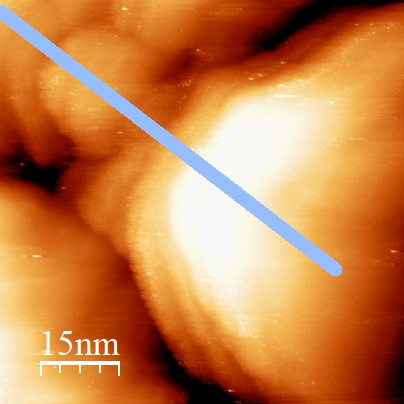
\includegraphics[scale=0.8]{Bilder/3000_IGain_vor.jpg}
\caption{Bild der z-Komponente bei Vermessung der Goldprobe mit einem I-Gain von 3000 in der Vorwärtsrichtung. Der Balken quer im Bild verbildlicht die Stelle, aus der das Höhenprofil entnommen wurde.}
\label{fig:Gold_IGain_Beispiel}
\end{figure}

\begin{figure}
\centering
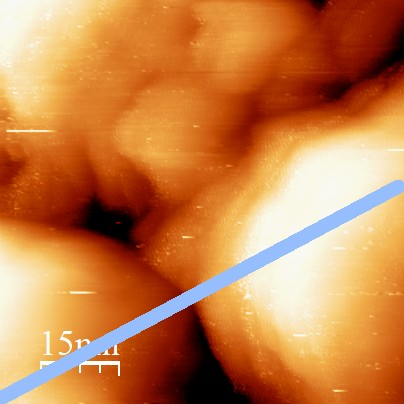
\includegraphics[scale=0.8]{Bilder/0_1_Zeit_vor.jpg}
\caption{Bild der z-Komponente bei Vermessung der Goldprobe bei einer Messzeit von 0,1s pro Linie in der Vorwärtsrichtung. Der Balken quer im Bild verbildlicht die Stelle, aus der das Höhenprofil entnommen wurde.}
\label{fig:Gold_Zeit_Beispiel}
\end{figure}

Abbildung \ref{fig:Gold_IGain_Beispiel} zeigt beispielhaft das Bild der z-Komponente nach Bearbeitung für eine Messung aus der Messreihe mit verändertem I-Gain. Der Balken quer im Bild zeigt, wo das im Folgenden untersuchte Höhenprofil entnommen wurde. In den Bildern aus den Ergebnissen der Messreihe wurde das Höhenprofil exakt gleich entnommen (Profillinie kopiert), sodass die Vergleichbarkeit der Profile gegeben ist.\\
Bei der Aufnahme der Messreihe mit veränderter Zeit wurde ein anderer Bereich verwendet. Daher ist die Profillinie aus einem anderen Bildbereich entnommen, wie in Abbildung \ref{fig:Gold_Zeit_Beispiel} dargestellt ist.\\
Bei der Entnahme des Höhenprofils wird für jeden Wert der Mittelwert mehrerer Punkte bestimmt.\\
Beide Messreihen wurden mit mehreren Methoden ausgewertet, die im Folgenden diskutiert werden.

\subsubsection{Bestimmung der Extremalpositionen}
Mit der Bestimmung der Positionen der Extremalstellen aus den Höhenprofilen bieten sich 2 Möglichkeiten zur Auswertung:
\begin{enumerate}
\item Die Verschiebung der Extremalstellen der Vorwärtsrichtung gegenüber den gleichen Peaks in der Rückrichtung ist bei zu großem I-Gain oder zu kleiner Zeit pro Linie sehr groß.
\item Mit den Positionen und Höhen der Extremalstellen kann die Flankensteigung bestimmt werden. Bei zu großem I-Gain oder zu kleiner Zeit pro Linie ist die Steigung zu groß und bei zu kleinem I-Gain zu klein.
\end{enumerate}

Für die Bestimmung der Positionen der Extremalstellen wurde ein Schätzwert aus den Profilen abgelesen und aus einem Bereich um diesen Schätzwert der Maximalwert gesucht. Wenn mehrere Punkte den gleichen (maximalen) Wert haben, wird zwischen diesen gemittelt.

\begin{figure}
\centering
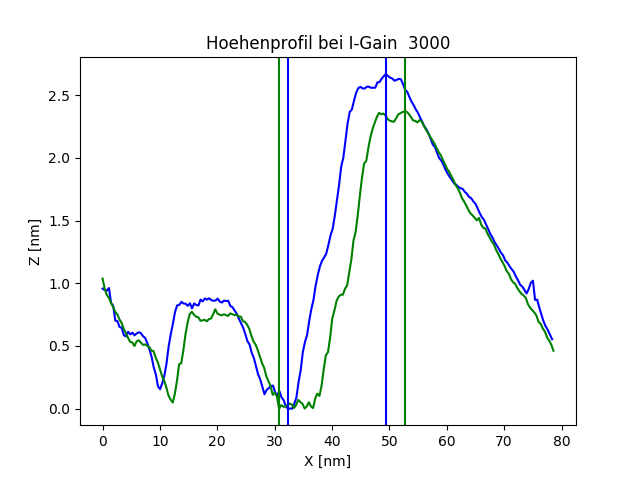
\includegraphics[scale=0.8]{Bilder/Profil_IGain_3000_Peakbestimmung.png}
\caption{Höhenprofil bei einem I-Gain von 3000 mit den durch senkrechte Linien markierten Extremalstellen. Das grüne Profil und entspricht der Vorwärts- und das blaue der Rückwärtsrichtung.}
\label{fig:Gold_IGain_Extremalstellen}
\end{figure}

\paragraph{Verschiebung der Extremalstellen}
Zur Bestimmung der Verschiebung der Extremalstellen wird einfach der Betrag der Abstände aufsummiert:
\begin{equation*}
\Sigma = \sum _{i = 0} ^n \, |x_i^{vor} - x_i^{rueck}|
\end{equation*}


\subsection{Untersuchung von HOPG}

\section{Fazit}

\section{Anhang}


\end{document}